\documentclass[11pt,oneside]{scrbook}
\usepackage[a4paper,margin=2.4cm,marginparwidth=1.8cm,marginparsep=0.4cm]{geometry}
\usepackage{../common/rlstudy}

\title{{\color{rlblue}\textbf{Week 23} \\ \Huge Safe Exploration, Shielding, CBFs, Robust RL}}
\author{STUDY-RL --- a self-paced Deep RL curriculum}
\date{\today}

\begin{document}
\maketitle
\tableofcontents
\newpage

\chapter*{Learning objectives}
\addcontentsline{toc}{chapter}{Learning objectives}


% Teaching companion: a small example before the full lecture.
\noindent\textbf{Study companion.} Read \texttt{teaching\_guide.md} in this
folder for step-by-step examples, an analogy with its limits, and self-checks.
Then use \texttt{workbook.ipynb} to implement and vary the calculations.
\par\medskip

\begin{keyidea}
By the end of this lecture you will be able to:
\begin{enumerate}[leftmargin=*]
  \item Express a safety property in Linear Temporal Logic (LTL) and translate
        it into a deterministic safety automaton.
  \item Synthesise a pre-shield from a safety automaton plus a one-step
        environment model; prove its soundness.
  \item Implement an LTL-shielded Q-learning loop in which the agent never
        commits an unsafe transition during training.
  \item State the safety-layer / differentiable-QP formulation
        (\textsc{Dalal et al.\ 2018}) and write down the closed-form
        projection for a single linear constraint.
  \item Derive the Control Barrier Function (CBF) condition and the
        per-step CBF--QP filter; reason about forward invariance.
  \item Compare domain randomisation, automatic domain randomisation (ADR),
        and adversarial training (RARL) as strategies for robust policy
        learning.
  \item Empirically demonstrate the OOD-generalisation benefit of domain
        randomisation on a pendulum task.
\end{enumerate}
\end{keyidea}

\chapter{Motivation \& intuition}

\section{When constraints don't go far enough}

Week 22's Lagrangian methods give us asymptotic constraint satisfaction --- in
the limit, $J_c(\pi^\star) \leq d$. But the policy is allowed to violate the
constraint along the way. For aerial vehicles, surgical robots, and
re-ranking systems with hard fairness mandates, ``asymptotic'' isn't enough.
We need to prevent unsafe transitions \emph{during training, including the
first episode}.

There are three classical families of techniques:
\begin{enumerate}[leftmargin=*]
  \item \textbf{Shielding} (Alshiekh et al.\ 2018, arXiv:1708.08611) ---
        a formal-methods construction: filter actions against a finite-state
        \emph{safety automaton} compiled from a temporal-logic spec.
  \item \textbf{Safety layers} (Dalal et al.\ 2018, arXiv:1801.08757) ---
        differentiable QP that projects the agent's action onto a half-space
        of safe actions.
  \item \textbf{Control barrier functions} (CBFs) --- a control-theoretic
        construction: define a function $h(s) \geq 0$ for the safe set and
        enforce a Lyapunov-style derivative condition.
\end{enumerate}

The common thread: \emph{decouple} the safety guarantee from the learning
algorithm. The agent can be anything --- Q-learning, PPO, SAC, a frozen
LLM-policy --- and the safety wrapper still works, with provable invariants.

\section{Robustness as a separate axis}

The second half of this week is \emph{robust} RL: making the policy
insensitive to perturbations of the environment dynamics. The two engineering
moves are
(i) \textbf{domain randomisation} (training on a distribution of environments
broad enough to cover the deployment one) and
(ii) \textbf{adversarial training} (a co-trained adversary perturbs the
dynamics to make the protagonist robust). Both reduce to ``don't overfit to
one dynamics function''.

\begin{intuition}
A shield resembles a railway interlock: a proposed move is checked against
a model of which moves preserve a specified invariant. Its guarantee depends
on that model and on the continued availability of a safe move.
Cross-validation, by contrast, estimates generalisation; it does not enforce it.
\end{intuition}

\chapter{Mathematical formulation}

\section{LTL primer}

\begin{definition}[LTL syntax]
Atomic propositions $p \in AP$ combine via Boolean connectives and the
temporal operators $\mathbf{X}$ (next), $\mathbf{G}$ (globally), $\mathbf{F}$
(eventually), $\mathbf{U}$ (until). The grammar is
\[
   \varphi \::=\: p \mid \neg \varphi \mid \varphi \wedge \varphi
              \mid \mathbf{X}\varphi \mid \varphi\, \mathbf{U}\, \varphi.
\]
$\mathbf{F}\varphi \defeq \top\, \mathbf{U}\, \varphi$ and
$\mathbf{G}\varphi \defeq \neg \mathbf{F}\neg\varphi$.
\end{definition}

The semantics is over infinite traces $w = w_0 w_1 \ldots$ of labels
$w_i \subseteq AP$. Key fragment for safety: the \emph{safety LTL} fragment
\[
   \mathbf{G}\, \psi(w_0, w_1, \ldots, w_k)
\]
of \emph{always}-properties on bounded windows. Every safety LTL formula
admits a deterministic finite automaton (DFA) on traces; violation is reaching
a designated rejecting sink.

\begin{example}[The lecture's running formula]
$\varphi = \mathbf{G}\, \neg \text{danger}$ --- ``never enter a danger cell''.
The DFA has two states $q_0$ (accepting, ``so far safe'') and $q_{bad}$
(rejecting, absorbing).
\end{example}

\section{Safety automaton and shield synthesis}

\begin{definition}[Safety automaton]
A safety automaton for $\varphi$ is $\mathcal{A}_\varphi = (Q, \Sigma, \delta,
q_0, F)$ with $\Sigma = 2^{AP}$, $\delta: Q \times \Sigma \to Q$, initial $q_0$
and accepting set $F \subseteq Q$. An infinite trace is accepted iff every
prefix lands in $F$.
\end{definition}

\begin{definition}[Pre-shield]\label{def:preshield}
Given a one-step environment model $M: \States \times \Actions \to \States$
and a safety automaton $\mathcal{A}_\varphi$, the \emph{pre-shield} maps each
$(s, q)$ to the safe action subset
\[
   \mathrm{safe}(s, q) \defeq \bigl\{\, a \in \Actions \;\big|\; \delta(q, L(M(s,a))) \in F \,\bigr\},
\]
where $L: \States \to 2^{AP}$ is the state-labelling function. The shielded
policy is $\pi_{\text{shielded}}(\cdot | s, q) \propto \pi(\cdot | s) \cdot \mathbb{1}_{\mathrm{safe}(s, q)}$.
\end{definition}

\begin{theorem}[Soundness of the pre-shield]\label{thm:shield-sound}
Suppose the environment is deterministic, $M$ is exact, and $\mathrm{safe}(s, q)$
is non-empty for every reachable $(s, q)$, the initial label is safe,
and the shielded sampler can assign positive mass to a safe action. Then every trajectory of the
shielded policy satisfies $\varphi$.
\end{theorem}

\begin{proof}
By induction on $t$. Base: $q_0 \in F$ by construction.
Step: at $(s_t, q_t)$ with $q_t \in F$, the shield by \cref{def:preshield}
picks $a_t$ such that $\delta(q_t, L(s_{t+1})) \in F$. So $q_{t+1} \in F$ and
the trace prefix of length $t+1$ is in $F^*$. Hence every prefix is in $F^*$,
which by definition of the safety automaton means the trace satisfies
$\varphi$.
\end{proof}

\begin{remark}
For stochastic dynamics a robust shield must check every possible successor
and keep the next state in a controllable safe set. For learned $M$,
additional coverage assumptions are required; soundness is not automatic: the shield is correct on the support of $M$, and
mis-modelling drives a violation probability. Learning-based shields
(\textsc{arXiv:2410.07359}, Oct 2024) bound this probability via concentration
inequalities on the learned model.
\end{remark}

\begin{pitfall}
\textbf{Empty safe set.} If at some $(s, q)$ the shield finds no safe action,
the next step may be unavoidable even though no violation has happened yet:
a one-step-safe move can enter a state from which every next move is unsafe. Standard recipes: (i) require an \emph{invariant
controller} that keeps the agent inside a known-controllable subset; (ii)
expand the spec to include a recovery clause; (iii) fail-safe by stopping.
\end{pitfall}

\section{Safety layer (Dalal et al.\ 2018)}

For continuous actions and a single linear constraint $g(s) + \nabla g(s)^\top a \leq 0$,
the safety layer solves
\[
   a^\star = \argmin_a \|a - a_\pi\|^2 \quad\text{s.t.}\quad g(s) + \nabla g(s)^\top a \leq 0.
\]
For a single linear constraint the closed-form projection is
\begin{equation}\label{eq:dalal-projection}
   a^\star = a_\pi - \max\!\left(0, \frac{g(s) + \nabla g(s)^\top a_\pi}{\|\nabla g(s)\|^2}\right) \nabla g(s).
\end{equation}
For multiple constraints, OptNet-style differentiable QPs (Amos \& Kolter
2017) make $\partial a^\star/\partial \theta$ usable as a backward layer.

\section{Control Barrier Functions}

\begin{definition}[CBF, control-affine systems]
For $\dot s = f(s) + g(s) a$, a continuously differentiable $h: \States \to \Real$
is a (zeroing) CBF for the safe set $\mathcal{C} = \{s : h(s) \geq 0\}$ if
there exists a class-$\mathcal{K}$ function $\alpha$ such that
\[
   \sup_{a \in \Actions} \bigl[\, \nabla h(s)^\top f(s) + \nabla h(s)^\top g(s)\, a \,\bigr] \;\geq\; -\alpha(h(s)).
\]
\end{definition}

\begin{theorem}[Forward invariance]\label{thm:cbf-invariance}
If $a(t)$ is any control law that for all $t$ satisfies
$\nabla h(s)^\top f(s) + \nabla h(s)^\top g(s)\, a \geq -\alpha(h(s))$, then
$h(s(t)) \geq 0$ for all $t \geq 0$ provided $h(s(0)) \geq 0$.
\end{theorem}

\begin{proof}[Proof sketch]
$\dot h \geq -\alpha(h)$ along trajectories. Comparison principle for ODEs:
$h(t) \geq y(t)$ where $y$ solves $\dot y = -\alpha(y), y(0) = h(0) \geq 0$.
Class-$\mathcal{K}$ $\alpha$ implies $y(t) \geq 0$ for all $t$, hence
$h(t) \geq 0$.
\end{proof}

The runtime safety filter is a per-step QP:
\begin{equation}\label{eq:cbf-qp}
   a^\star(s) = \argmin_a \|a - a_\pi(s)\|^2
   \quad\text{s.t.}\quad \nabla h(s)^\top g(s) a \geq -\alpha(h(s)) - \nabla h(s)^\top f(s).
\end{equation}
For a 1-D constraint this is again the closed-form projection of
\cref{eq:dalal-projection}, with $g(s) := \nabla h(s)^\top g(s)$ and
$b := -\alpha(h(s)) - \nabla h(s)^\top f(s)$.

\begin{remark}
HJ-reachability and CBF are duals: HJ gives the largest CBF-like function
analytically by solving an HJI PDE; CBF chooses a simpler analytic $h$ and
checks the inequality. \textsc{arXiv:2204.12507} (2022, extended 2024)
iteratively refines $h$ using HJ.
\end{remark}

\section{Robust RL: domain randomisation and adversarial training}

\begin{definition}[Robust MDP]\label{def:robust-mdp}
A Robust MDP $(\States, \Actions, \mathcal{U}, r, \gamma)$ replaces the
transition kernel by an \emph{uncertainty set} $\mathcal{U}$. The robust
value is
\[
   V^\pi_{\text{rob}}(s) = \inf_{P \in \mathcal{U}}\; \E_{\pi, P}\!\left[\sum_t \gamma^t r(s_t, a_t) \,\bigg|\, s_0 = s\right].
\]
\end{definition}

For \emph{rectangular} $\mathcal{U}$ (i.e.\ independent uncertainty for each
$(s, a)$) the robust Bellman operator $T_{\text{rob}}$ is a $\gamma$-contraction,
so robust value iteration converges (\textsc{Iyengar 2005}; \textsc{Nilim \&
El Ghaoui 2005}).

\textbf{Domain randomisation} (DR; \textsc{Tobin et al.\ 2017}, arXiv:1703.06907)
side-steps the inner $\inf_P$ by sampling $P \sim \mathcal{D}$ during training
and maximising the \emph{average} return. This is robust-on-average rather
than robust-worst-case, but in practice frequently outperforms more careful
robust algorithms for sim-to-real.

\textbf{ADR} (Automatic Domain Randomisation; OpenAI 2019, arXiv:1910.07113)
expands $\mathcal{D}$'s support whenever the agent's performance on the
boundary parameters becomes good --- a curriculum on randomness.

\textbf{RARL} (\textsc{Pinto et al.\ 2017}) plays a zero-sum game between a
protagonist policy and a disturbance policy that perturbs the dynamics. At a
Nash equilibrium the protagonist is robust to bounded adversarial perturbations.

\chapter{Algorithms}

\section{Shielded Q-learning pseudocode}

\begin{tcolorbox}[colback=mintedbg, colframe=rlgray!50, title=\textbf{Algorithm: Shielded Q-learning (one episode)}]
\textbf{Inputs:} env $\mathcal{M}$, agent $Q$, shield with predicate
$\mathrm{unsafe}(s, a)$.
\begin{enumerate}[leftmargin=*]
  \item Reset env; $s \leftarrow s_0$.
  \item Until done:
  \begin{enumerate}
    \item Build $\epsilon$-greedy preference list $\sigma$ over actions.
    \item Filter: $a \leftarrow \text{first}\, a \in \sigma$ with $\neg\mathrm{unsafe}(s, a)$.
    \item Step env: $(s', r, \text{done}) = \mathcal{M}.\text{step}(a)$.
    \item Update: $Q(s, a) \leftarrow Q(s, a) + \alpha (r + \gamma \max_{a'} Q(s', a') - Q(s, a))$.
    \item $s \leftarrow s'$.
  \end{enumerate}
\end{enumerate}
\textbf{Invariant:} the trace never visits a danger cell (\cref{thm:shield-sound}).
\end{tcolorbox}

\section{Safety-layer pseudocode (continuous control)}

\begin{tcolorbox}[colback=mintedbg, colframe=rlgray!50, title=\textbf{Algorithm: Safety layer wrapper}]
\begin{enumerate}[leftmargin=*]
  \item Forward through actor: $a_\pi = \pi_\theta(s)$.
  \item Compute $g(s)$ (constraint value) and $\nabla g(s)$ (its gradient).
  \item Project: $a = a_\pi - \max(0, (g + \nabla g^\top a_\pi)/\|\nabla g\|^2) \nabla g$.
  \item Step env with $a$; record $(s, a, r, s')$; backprop through the
        projection.
\end{enumerate}
\end{tcolorbox}

\section{Domain randomisation training}

\begin{tcolorbox}[colback=mintedbg, colframe=rlgray!50, title=\textbf{Algorithm: DR-PG (one epoch)}]
\begin{enumerate}[leftmargin=*]
  \item Sample $T$ rollouts; for each rollout, sample env parameters
        $\eta \sim \mathcal{D}$ at reset (e.g.\ pole length).
  \item Compute Monte-Carlo returns and advantages with a value baseline.
  \item PG step: $\theta \leftarrow \theta + \alpha \nabla_\theta \E_{\eta, \pi_\theta}[\log \pi_\theta\, A]$.
\end{enumerate}
\end{tcolorbox}

\begin{pitfall}
\textbf{DR plateau.} If $\mathcal{D}$ is too broad, the gradient signal becomes
the average of many incompatible policies --- the agent learns nothing.
Symptom: training return barely improves. Fix: start narrow, widen via ADR
once the easy region is solved.
\end{pitfall}

\chapter{Implementation walkthrough}

\section{The danger gridworld and its DFA}

\begin{minted}{python}
@dataclass
class DangerGridWorld:
    rows: int = 5; cols: int = 5
    start = (0, 0); goal = (4, 4)
    danger = ((1,2),(2,1),(2,2),(2,3),(3,2))
    def label(self, s_idx):
        return {"danger"} if self.idx2s(s_idx) in self.danger_set else set()
    def adjacent_dangerous(self, s_idx, a):
        # one-step lookahead — deterministic, so this is the complete model
        ...
\end{minted}

The DFA has two states (\cref{fig:dfa}). The shield in \texttt{shield.py}
implements the action filter: it iterates over preferred actions (ordered by
Q-value, or by epsilon-greedy randomisation), returns the first action whose
one-step image stays in $q_0$, and counts the number of overrides.

\section{Q-learning under the shield}

\begin{minted}{python}
def act(self, s, ep, shield=None):
    if rng.random() < eps(ep):
        order = list(rng.permutation(self.n_actions))
    else:
        order = list(np.argsort(-self.Q[s]))
    if shield is not None:
        return shield.filter(s, order)
    return order[0]
\end{minted}

Crucial design choice: the shield is applied \emph{inside the epsilon-greedy
sampler}, not after. This means exploration is also shield-compliant; the
$\epsilon$-greedy random action is replaced by a random \emph{safe} action.

\section{Pendulum with DR}

\begin{minted}{python}
@dataclass
class PendulumDR:
    randomise: bool = True
    length_low: float = 0.5; length_high: float = 1.5
    def reset(self, seed=None):
        ...
        if self.randomise:
            self.length = self.rng.uniform(self.length_low, self.length_high)
\end{minted}

The state observation is $[\cos\theta, \sin\theta, \dot\theta]$ --- no
length channel --- so the policy must implicitly handle the dynamics
variation.

\section{Robustness comparison}

The training loop runs REINFORCE with a value baseline (no policy
distribution information about the length is given). At test time we
evaluate at fixed lengths $\{0.3, 0.6, 1.0, 1.4, 1.8\}$. The DR policy was
trained on $[0.5, 1.5]$ so $0.3$ and $1.8$ are mild OOD points; the fixed
policy was trained at $1.0$ so all but the centre are OOD.

\chapter{Empirical results}

\begin{figure}[h]
  \centering
  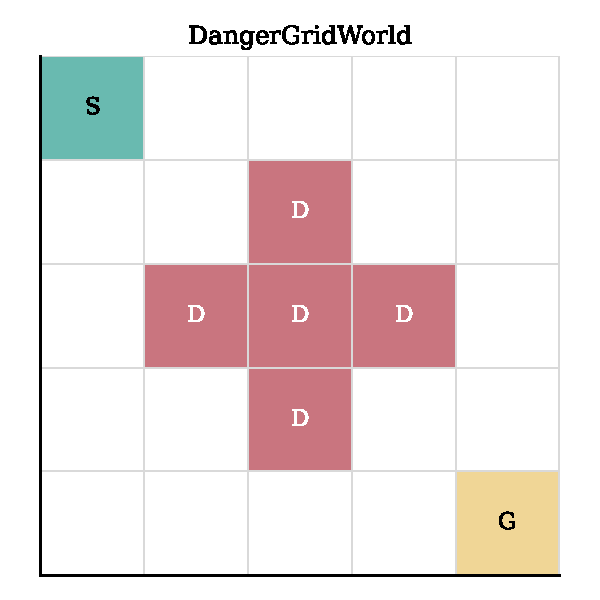
\includegraphics[width=0.45\linewidth]{figs/fig_grid.pdf}\hfill
  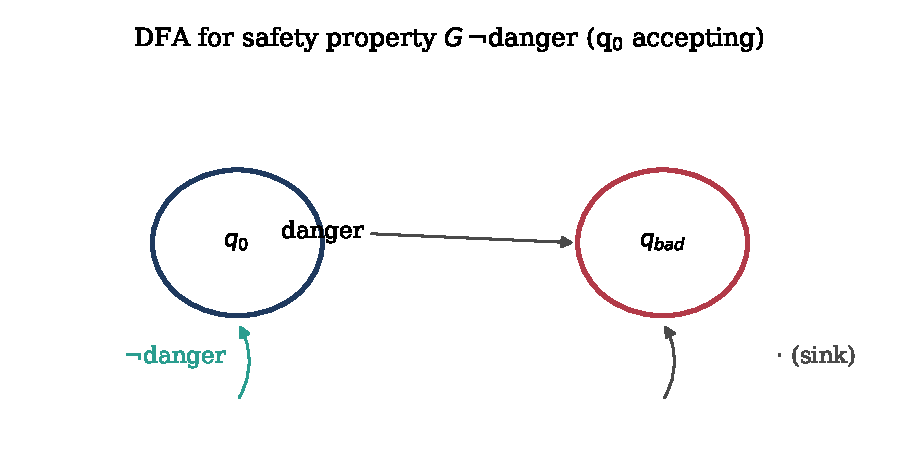
\includegraphics[width=0.5\linewidth]{figs/fig_dfa.pdf}
  \caption{Left: the danger gridworld used for the shielded Q-learning
  demo. Right: the two-state safety automaton for $\mathbf{G}\,\neg$danger.}
  \label{fig:dfa}
\end{figure}

\begin{figure}[h]
  \centering
  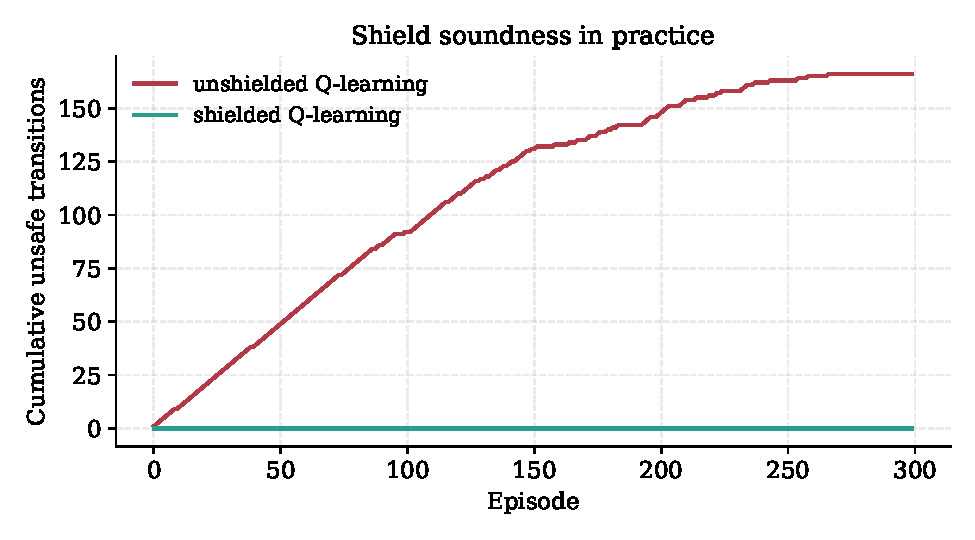
\includegraphics[width=0.5\linewidth]{figs/fig_unsafe_curve.pdf}\hfill
  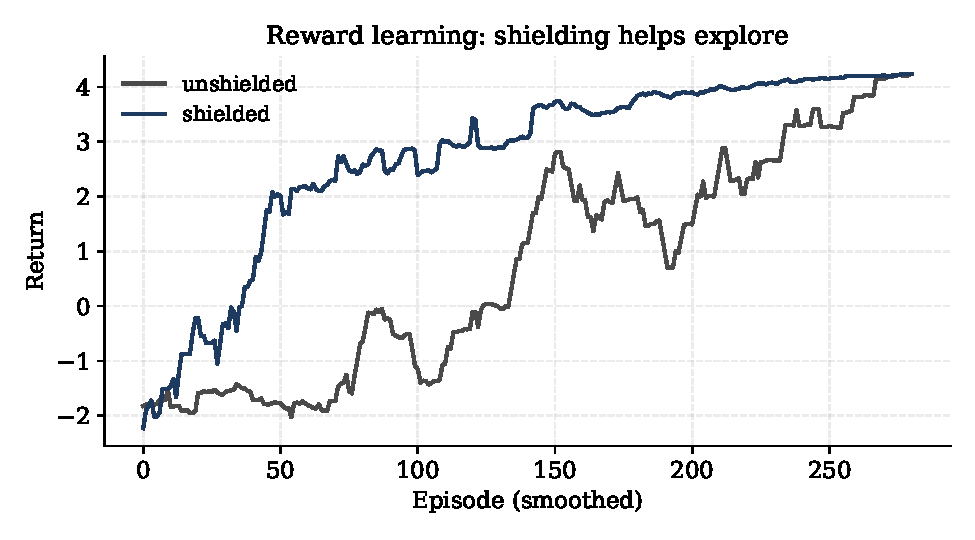
\includegraphics[width=0.49\linewidth]{figs/fig_return_curve.pdf}
  \caption{Left: cumulative unsafe transitions. The shielded curve sits at
  zero throughout (\cref{thm:shield-sound}). Right: smoothed episodic
  return. The shielded agent learns at least as fast as the unshielded
  baseline --- the shield's overrides serve as ``free'' exploration into
  unsafe regions without actually visiting them.}
  \label{fig:safety-curves}
\end{figure}

\begin{figure}[h]
  \centering
  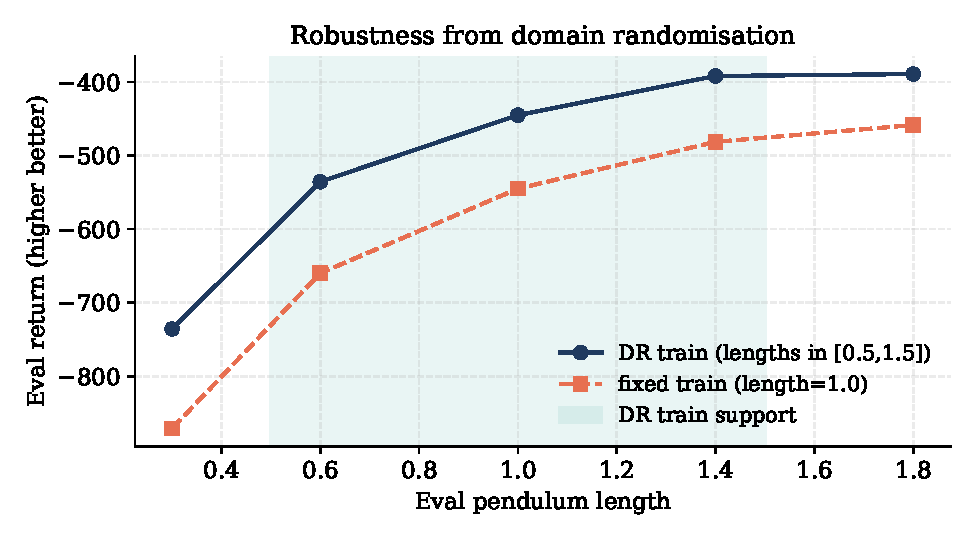
\includegraphics[width=0.75\linewidth]{figs/fig_pendulum_dr.pdf}
  \caption{DR vs.\ fixed-length training, evaluated at a range of test
  lengths. Shaded region is the DR training support. The fixed-length policy
  collapses on OOD lengths; the DR policy degrades gracefully even outside
  its training distribution.}
  \label{fig:dr}
\end{figure}

\begin{safetyangle}
This is, ultimately, the chapter about \emph{deployment}. The lecture's
running message:
\begin{itemize}[leftmargin=*]
  \item \textbf{Shielding handles known-knowns.} If you have written down
        what ``safe'' means, you can synthesise a shield. If you haven't,
        no shield will save you.
  \item \textbf{Robust training handles known-unknowns.} DR makes the policy
        less brittle to dynamics you can enumerate (mass, friction, sensor
        noise). It does nothing for unknown-unknowns.
  \item \textbf{Composition matters.} In production we typically stack:
        offline-pretrained policy + Lagrangian-fine-tuned policy + CBF runtime
        filter + monitoring. Each layer addresses a different failure mode.
\end{itemize}
References: \textsc{Alshiekh et al.\ 2018}, arXiv:1708.08611, ``Safe RL via
Shielding''; \textsc{Dalal et al.\ 2018}, arXiv:1801.08757, ``Safe exploration
in continuous action spaces''; \textsc{Tobin et al.\ 2017}, arXiv:1703.06907,
``Domain randomization for sim-to-real transfer''. The 2024-2025 update is
\textsc{arXiv:2410.07359} on learning-based shielding under unknown dynamics,
and \textsc{arXiv:2502.13187} for foundation-model-conditioned sim-to-real.
\end{safetyangle}

\begin{matching}
For synthetic ATS candidate-matching: a shield can enforce hard regulatory
constraints (e.g.\ ``never present a candidate whose audit flag is RED''),
operating as a post-filter on the ranking policy's top-$K$ output. The
``state'' is the current shortlist plus the candidate under consideration;
the safety automaton is the verbalised hiring policy compiled into a
checker.

For synthetic insurance lead-matching, a CBF-style filter caps a single broker's daily
allocation: $h(s) = q_{max} - n_{assigned}(s) \geq 0$. The runtime QP enforces
the cap in real time, no matter what the underlying ranking model wants.

Domain randomisation generalises to \emph{population shift}: train the
re-ranker on a randomised mix of recruiter-quality profiles, candidate-supply
shapes, and seasonal cohorts. The resulting policy is robust to month-to-month
distribution drift in the live system without retraining.
\end{matching}

\chapter{Exercises}
See \texttt{workbook.ipynb} for graded exercises with hints:
\begin{itemize}[leftmargin=*]
  \item \textbf{Ex.\ 1 ($\star$):} build the DFA for $\mathbf{G}\,\neg$danger.
  \item \textbf{Ex.\ 2 ($\star$):} unsafe-predicate one-step look-ahead.
  \item \textbf{Ex.\ 3 ($\star\star$):} implement the pre-shield filter.
  \item \textbf{Ex.\ 4 ($\star\star$):} shielded vs unshielded Q-learning.
  \item \textbf{Ex.\ 5 ($\star\star$):} verify shield soundness empirically.
  \item \textbf{Ex.\ 6 ($\star\star$):} DR vs fixed-length pendulum (meaningful objective).
  \item \textbf{Ex.\ 7 ($\star\star\star$):} 1-D CBF projection in closed form.
  \item \textbf{Ex.\ 8 ($\star\star\star$):} adversarial-extreme OOD evaluation.
\end{itemize}

\chapter{Further reading}
See \texttt{extended\_reading.pdf}. Sourced from
\texttt{research/safety\_rl\_sota.md} sections 2, 4, 9.

\end{document}
